\documentclass[11pt,a4paper]{article}

% ==============================================================================
% COMPATIBILIDAD AUTOMÁTICA CON PDFLATEX (Overleaf / TeXLive) Y XELATEX
% ==============================================================================
\usepackage{iftex}
\ifPDFTeX
  \usepackage[utf8]{inputenc}
  \usepackage[T1]{fontenc}
  \usepackage{lmodern}
\else
  \usepackage{fontspec}
\fi

\usepackage[spanish,es-tabla]{babel}
\usepackage[a4paper,top=1.9cm,bottom=1.9cm,left=2.0cm,right=2.0cm]{geometry}
\usepackage{amsmath,amssymb}
\usepackage{graphicx}
\usepackage{subcaption}
\usepackage{booktabs}
\usepackage{array}
\usepackage{float}
\usepackage{enumitem}
\usepackage{xcolor}
\usepackage{fancyhdr}
\usepackage{titlesec}
\usepackage{microtype}
\usepackage[hidelinks,hypertexnames=false]{hyperref}

% ==============================================================================
% COLORES CORPORATIVOS UNIVERSIDAD DE SEVILLA
% ==============================================================================
\definecolor{burdeosUS}{HTML}{9D2235} % Pantone 201 CVC
\definecolor{alberoUS}{HTML}{FFC72C}  % Pantone 123 CVC
\definecolor{grisTexto}{HTML}{333333}

% Estilo de títulos de secciones
\titleformat{\section}
  {\large\bfseries\color{burdeosUS}}{\thesection.}{0.6em}{}[\color{alberoUS}\titlerule]
\titleformat{\subsection}
  {\normalsize\bfseries\color{burdeosUS}}{\thesubsection.}{0.5em}{}

\titlespacing*{\section}{0pt}{10pt plus 2pt minus 2pt}{4pt}
\titlespacing*{\subsection}{0pt}{7pt plus 2pt minus 2pt}{2pt}

% Encabezado y pie de página
\pagestyle{fancy}
\fancyhf{}
\fancyhead[L]{\small\color{gray}Teoría de Grafos aplicada a Twitch — MATI}
\fancyhead[R]{\small\color{gray}Universidad de Sevilla, II - TI}
\fancyfoot[C]{\small\color{gray}\thepage}
\renewcommand{\headrulewidth}{0.4pt}

% Ajustes tipográficos para evitar cortes feos y desbordes de margen
\setlength{\parskip}{0.32em}
\setlength{\parindent}{0pt}
\setlength{\textfloatsep}{8pt plus 2pt minus 2pt}
\setlength{\intextsep}{8pt plus 2pt minus 2pt}
\setlength{\emergencystretch}{3em}
\clubpenalty=10000
\widowpenalty=10000
\displaywidowpenalty=10000

% ==============================================================================
% INICIO DEL DOCUMENTO
% ==============================================================================
\begin{document}

% --- PÁGINA 1: PORTADA OFICIAL ---
\begin{titlepage}
    \centering
    \vspace*{1cm}

    {\large \textsc{Universidad de Sevilla} \par}
    \vspace{0.2cm}
    {\normalsize Escuela Técnica Superior de Ingeniería Informática \par}
    {\normalsize Grado en Ingeniería Informática -- Tecnología Informática \par}

    \vspace{1.2cm}
    {\color{burdeosUS}\rule{\linewidth}{2.2pt}}
    \vspace{0.8cm}

    {\LARGE \bfseries \color{burdeosUS}
    Teoría de Grafos aplicada a Twitch:\\[0.3em]
    Centralidad, Comunidades y Evolución Estructural \par}

    \vspace{0.5cm}
    {\large \itshape Memoria del proyecto de asignatura \par}

    \vspace{0.8cm}
    {\color{alberoUS}\rule{0.6\linewidth}{2pt}}

    \vspace{2.2cm}

    {\large \textbf{Asignatura} \par}
    \vspace{0.2cm}
    {Matemática Aplicada a las Tecnologías de la Información (MATI) \par}

    \vspace{1.6cm}

    {\large \textbf{Autores} \par}
    \vspace{0.4cm}
    \begin{tabular}{c}
        Francisco José Caballero Mesa \\[0.25em]
        Andrea Cárdenas Mayoral \\[0.25em]
        Marco Granja Quinto \\[0.25em]
        Moisés Guillermo Godoy Nava \\[0.25em]
        Alberto López López
    \end{tabular}

    \vfill

    {\color{burdeosUS}\rule{0.4\linewidth}{0.8pt}}\\[0.5em]
    {\large Sevilla, 30 de noviembre de 2026 \par}
\end{titlepage}

% --- PÁGINA 2: ÍNDICE ---
\pagenumbering{roman}
\tableofcontents
\newpage
\pagenumbering{arabic}

% ==============================================================================
\section{Introducción, artículo de partida y objetivos}
% ==============================================================================

En la sociedad actual existen numerosas redes sociales en las que distintos usuarios retransmiten contenido que millones de personas consumen en tiempo real. Entre ellas destaca \textbf{Twitch}, una plataforma de retransmisión en directo que en los últimos años ha experimentado un enorme crecimiento en audiencia, pasando de ser un espacio enfocado en videojuegos a consolidarse como uno de los principales medios de entretenimiento digital. Al tratarse de un ecosistema donde interactúan creadores y espectadores a gran escala, resulta especialmente interesante analizar sus relaciones mediante la teoría de grafos para entender cómo se concentra la popularidad, cómo se articulan las comunidades y qué usuarios resultan estructuralmente decisivos.

El punto de partida de este trabajo es el artículo \textit{Twitch Gamers: a Dataset for Evaluating Proximity Preserving and Structural Role-based Node Embeddings} (Rozemberczki y Sarkar, 2021)~\cite{rozemberczki2021}, publicado en la colección SNAP de la Universidad de Stanford. Dicho conjunto de datos recoge las relaciones de seguimiento mutuo entre $168\,114$ cuentas de Twitch etiquetadas en $21$ idiomas (con $6\,797\,557$ enlaces), junto con atributos reales de cada canal, como sus visualizaciones acumuladas, antigüedad, contenido adulto, estatus de afiliado o si la cuenta está inactiva.

A partir de este estudio base, planteamos tres bloques de preguntas de investigación:
\begin{enumerate}[leftmargin=*, itemsep=2pt]
  \item \textbf{Topología interna y centralidad:} ¿Cómo se reparte la popularidad dentro de una comunidad lingüística? ¿Qué usuarios resultan más importantes según distintas medidas de centralidad? ¿Cómo resiste la red ante fallos aleatorios frente a ataques dirigidos?
  \item \textbf{Dimensión lingüística:} ¿Cambia la estructura de la red según el idioma? ¿Actúa la lengua como una frontera natural entre comunidades?
  \item \textbf{Evolución temporal y cambio de perspectiva de los datos:} ¿Cómo cambia la estructura observada de Twitch entre 2018 y 2026 cuando pasamos de estudiar seguimientos mutuos (SNAP 2018) a analizar audiencia compartida en directo (Kaggle Live 2019, GitHub Overlap 2021--2022 y nuestra captura propia de noviembre de 2026)? ¿Qué parte de ese cambio responde a la evolución real de la plataforma y qué parte a la distinta definición de arista tras el cierre de la función de amigos y de las listas públicas de seguidores?
\end{enumerate}

Desde el punto de vista metodológico, aplicamos de forma estricta la verificación previa de precondiciones antes de lanzar cualquier algoritmo (comprobando simplicidad, conexidad y alineación de índices en matrices) para evitar resultados erróneos o sin sentido. Todo el análisis computacional se realiza en \textit{SageMath}, apoyándonos puntualmente en \textit{NetworkX} (la librería de Python para análisis de redes complejas integrada en el mismo entorno) para acelerar métricas como la centralidad de autovector o la detección de comunidades, y se completa con demostraciones constructivas y una aplicación interactiva divulgativa.

% ==============================================================================
\section{Modelización matemática y comprobaciones previas}
% ==============================================================================

Modelamos la red de seguimiento mutuo de SNAP 2018~\cite{rozemberczki2021} como un grafo simple no dirigido $G = (V, A)$, donde cada vértice $v \in V$ representa una cuenta y cada arista $\{u,v\} \in A$ indica una relación de seguimiento recíproco (evitando llamarla «amistad» en sentido personal). Analizar de forma exacta los $168\,114$ vértices globales, dominados por el inglés (\texttt{EN}) con $124\,411$ usuarios, resulta computacionalmente prohibitivo para algoritmos exactos de complejidad $O(n \cdot m)$ o espectrales en un ordenador estándar. Por ello, extraemos dos subgrafos inducidos completos e independientes de distinta escala para contrastar su comportamiento, correspondientes a los idiomas \textbf{portugués (\texttt{PT})} y \textbf{español (\texttt{ES})}. Conviene recalcar que el campo \texttt{language} refleja el idioma de emisión y no un único país, ya que \texttt{PT} agrupa principalmente a usuarios de Brasil y Portugal, mientras que \texttt{ES} reúne a España y Latinoamérica.

Antes de calcular métricas de distancia o centralidad, ejecutamos un protocolo formal de comprobaciones previas sobre cada subgrafo:
\begin{itemize}[leftmargin=*, itemsep=2pt]
  \item \textbf{Grafo simple y Lema del apretón de manos:} Se verifica computacionalmente la ausencia de lazos y aristas múltiples (\texttt{has\_loops() == False}, \texttt{has\_multiple\_edges() == False}) y el cumplimiento exacto de $\sum_{v \in V} \delta(v) = 2|A|$, tanto en \texttt{PT} ($85\,904 = 2 \times 42\,952$) como en \texttt{ES} ($171\,786 = 2 \times 85\,893$).
  \item \textbf{Dispersión y estructura de datos:} La densidad observada es muy baja, con un $1,336\%$ en \texttt{PT} y un $0,529\%$ en \texttt{ES}. Al tratarse de grafos dispersos ($|A| \ll n^2$), representarlos mediante \textbf{listas de adyacencia} ($O(n + |A|)$) evita malgastar memoria. Asimismo, para calcular la centralidad de Bonacich en \texttt{ES} ($5\,524$ nodos), usar matrices dispersas en formato CSC (\texttt{scipy.sparse}) evita reservar unos $244$\,MB de ceros y resuelve el sistema lineal en menos de un segundo.
  \item \textbf{Conexidad y Teorema de Whitney:} Al comprobar \texttt{is\_connected()}, detectamos que \textbf{ninguno de los dos subgrafos es conexo}. El subgrafo \texttt{PT} tiene $93$ componentes conexas ($90$ vértices aislados y dos parejas aisladas) y \texttt{ES} tiene $169$ componentes ($161$ aislados). Esos usuarios aislados no carecen de enlaces en el Twitch global, sino que seguían a cuentas de otros idiomas y sus aristas desaparecieron al inducir el subgrafo. Al tener grado mínimo $\delta(G) = 0$, el \textbf{Teorema de Whitney} ($\kappa(G) \le \lambda(G) \le \delta(G)$) garantiza $\kappa(G) = \lambda(G) = 0$. Para evitar distancias infinitas, restringimos las métricas basadas en caminos a la \textbf{componente conexa gigante propia de cada subgrafo}. En \texttt{PT}, $G_{\text{gig, PT}}$ agrupa al $96,29\%$ de los usuarios ($2\,442$ nodos) y cuenta con $108$ vértices de corte y $136$ aristas puente; en \texttt{ES}, $G_{\text{gig, ES}}$ reúne al $96,93\%$ ($5\,524$ nodos), con $252$ vértices de corte y $295$ puentes. En ambas componentes gigantes se cumple $\kappa(G_{\text{gig}}) = \lambda(G_{\text{gig}}) = \delta(G_{\text{gig}}) = 1$.
\end{itemize}

\begin{table}[H]
\centering
\caption{Principales medidas topológicas de las comunidades de portugués (\texttt{PT}) y español (\texttt{ES}) en 2018.}
\label{tab:pt_es}
\footnotesize
\renewcommand{\arraystretch}{0.95}
\begin{tabular}{@{}lcc@{}}
\toprule
\textbf{Medida topológica} & \textbf{Portugués (\texttt{PT}, 2018)} & \textbf{Español (\texttt{ES}, 2018)} \\
\midrule
Vértices $|V|$ & $2\,536$ & $5\,699$ \\
Aristas internas $|A|$ & $42\,952$ & $85\,893$ \\
Densidad & $1,336\%$ & $0,529\%$ \\
Grado medio (y mediana) & $33,87$ (mediana $17,0$) & $30,14$ (mediana $14,0$) \\
Grado máximo (mayor \textit{hub}) & $880$ & $1\,131$ \\
Coeficiente de variación del grado ($CV$) & $1,838$ & $1,934$ \\
Usuarios aislados (componentes totales) & $90$ ($93$ comp.) & $161$ ($169$ comp.) \\
Componente gigante $G_{\text{gig}}$ & $2\,442$ ($96,29\%$) & $5\,524$ ($96,93\%$) \\
Vértices de corte y puentes ($G_{\text{gig}}$) & $108$ vértices, $136$ puentes & $252$ vértices, $295$ puentes \\
Radio y diámetro de $G_{\text{gig}}$ & Radio $4$, diámetro $7$ & Radio $4$, diámetro $8$ \\
Tamaño del Centro $Z(G_{\text{gig}})$ & $144$ vértices & $4$ vértices \\
Distancia media (BFS, $150$ orígenes) & $2,641$ saltos & $2,872$ saltos \\
Clustering real (frente a \texttt{GNP}) & $0,3031$ ($22,3\times$ azar) & $0,2247$ ($40,9\times$ azar) \\
Afectados por Paradoja de la Amistad & $93,9\%$ & $95,0\%$ \\
Comunidades (\textit{greedy}) y modularidad $Q$ & $15$ ($Q = 0,2529$) & $31$ ($Q = 0,3862$) \\
Número de triángulos ($C_3$) & $262\,853$ & $400\,497$ \\
Clique máximo en el núcleo (Top 150) & $K_{18}$ & $K_{18}$ \\
Spearman grado vs.\ \texttt{views} & $\rho = +0,5994$ & $\rho = +0,5627$ \\
Spearman grado vs.\ \texttt{dead\_account} & $\rho = -0,2061$ & $\rho = -0,1294$ \\
\bottomrule
\end{tabular}
\end{table}

% ==============================================================================
\section{Distribución de grados, Efecto Mateo y modelos generadores}
% ==============================================================================

La Tabla~\ref{tab:pt_es} muestra una fuerte desigualdad en cómo se reparten las conexiones. En ambos idiomas el grado medio duplica a la mediana, situándose en $33,87$ frente a $17,0$ en \texttt{PT}, y en $30,14$ frente a $14,0$ en \texttt{ES}. El coeficiente de variación roza el valor $2$ ($CV = 1,838$ y $1,934$), reflejando la presencia de grandes concentradores (\textit{hubs}) que alcanzan hasta $880$ enlaces internos en \texttt{PT} y $1\,131$ en \texttt{ES}.

\subsection{Elección de modelos y ajuste por mínimos cuadrados}
Al representar en un gráfico el grado de cada usuario frente al número de usuarios con ese grado (Figura~\ref{fig:ajustes_es}), se observa una caída muy brusca al principio seguida de una cola larga pegada al eje horizontal. Esto descarta de inmediato un modelo lineal, ya que las frecuencias no decrecen a ritmo constante, y conduce a probar familias de funciones decrecientes vistas en clase, empezando por un \textbf{modelo exponencial} ($a e^{bx}$), pasando a una \textbf{ley de potencias pura} ($a x^b$) y terminando con una \textbf{ley de potencias desplazada} ($a |x - c|^b$).

Para ajustar los parámetros se utiliza \texttt{find\_fit} en \textit{SageMath}, que minimiza el error cuadrático total ($\text{SSE}$). Elevar cada diferencia al cuadrado evita que los errores positivos y negativos se cancelen entre sí y penaliza más las desviaciones grandes. En el modelo desplazado se introduce el valor absoluto $|x - c|^b$ y un punto inicial coherente (\texttt{initial\_guess}) para impedir que, durante las pruebas internas del optimizador, una base negativa elevada a un exponente fraccionario produzca un error de dominio. Los resultados obtenidos son:
\begin{itemize}[leftmargin=*, itemsep=2pt]
  \item \textbf{Subgrafo \texttt{PT}:} Potencial Puro $\text{SSE} = 14\,984,01$ ($b = -0,629$); Exponencial $\text{SSE} = 3\,469,86$; \textbf{Potencial Desplazado} $\text{SSE} = \mathbf{2\,677,55}$ ($a = 3,90\times 10^6$, $b = -2,825$, $c = -39,29$).
  \item \textbf{Subgrafo \texttt{ES}:} Potencial Puro $\text{SSE} = 121\,535,01$; Exponencial $\text{SSE} = 8\,285,93$; \textbf{Potencial Desplazado} $\text{SSE} = \mathbf{4\,443,64}$ ($a = 3,31\times 10^8$, $b = -3,642$, $c = -44,17$).
\end{itemize}

Los dos primeros modelos se descartan por motivos complementarios. El \textbf{exponencial} acompaña bien la bajada inicial, pero cae demasiado rápido hacia cero y es incapaz de explicar la cola larga donde aparecen los \textit{hubs}. Por su parte, el \textbf{potencial puro} dispara su error porque exige una asíntota vertical pegada a $k = 1$, mientras que en los subgrafos inducidos los grados bajos ($k < 15$) aparecen achatados al perderse los enlaces con otros idiomas. El \textbf{potencial desplazado} corrige ambos problemas a la vez, ya que el parámetro $c$ absorbe el desfase de los grados pequeños y conserva la cola pesada, logrando el menor error cuadrático y confirmando el \textbf{Efecto Mateo}. Siguiendo a Clauset, Shalizi y Newman (2009)~\cite{clauset2009}, conviene precisar que el ajuste por mínimos cuadrados es una herramienta descriptiva útil, aunque probar una ley de potencias estricta requeriría contrastes de máxima verosimilitud sobre la cola.

\begin{figure}[H]
  \centering
  \begin{subfigure}[b]{0.48\textwidth}
    \centering
    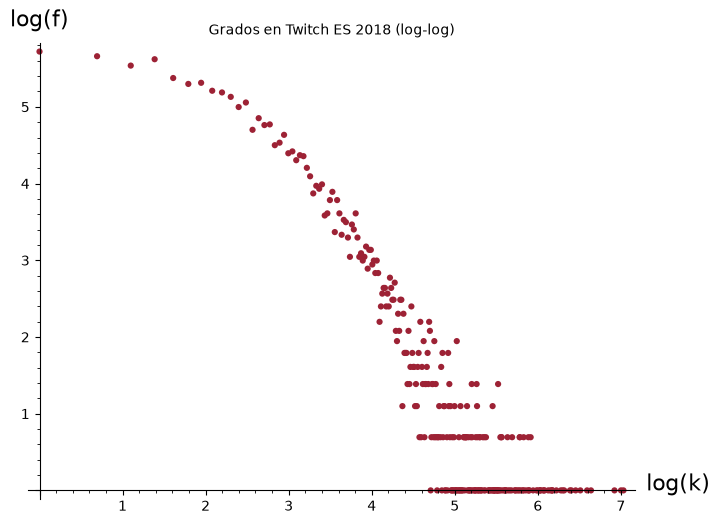
\includegraphics[width=\textwidth]{datos/salidas/grafica_ES_1_loglog.png}
    \caption{Distribución de grados en escala log-log.}
  \end{subfigure}
  \hfill
  \begin{subfigure}[b]{0.48\textwidth}
    \centering
    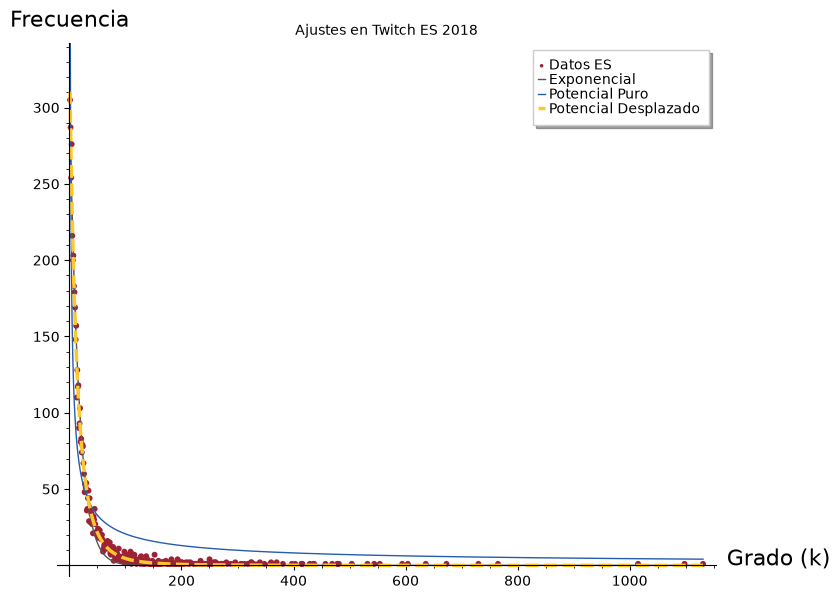
\includegraphics[width=\textwidth]{datos/salidas/grafica_ES_2_ajustes.png}
    \caption{Ajustes por mínimos cuadrados (\texttt{find\_fit}).}
  \end{subfigure}
  \caption{Análisis de la distribución de grados en el subgrafo de español (\texttt{ES}, 2018).}
  \label{fig:ajustes_es}
\end{figure}

\subsection{Paradoja de la Amistad y comparativa con modelos aleatorios}
\textbf{La Paradoja de la Amistad se cumple de forma abrumadora} en las dos comunidades analizadas. En \texttt{PT}, el \textbf{$93,9\%$} de los usuarios tiene menos conexiones mutuas que el promedio de sus propios contactos, y en \texttt{ES} la proporción sube al \textbf{$95,0\%$}. Es decir, más de $9$ de cada $10$ usuarios están menos conectados que la media de la gente con la que se enlazan. Matemáticamente es consecuencia directa de la desigualdad de Cauchy--Schwarz ($\langle \delta_{\text{vecinos}} \rangle = \bar{\delta} + \sigma_\delta^2 / \bar{\delta}$), puesto que al existir una varianza de grados ($\sigma_\delta^2$) tan elevada, los grandes \textit{hubs} figuran en los vecindarios de cientos de cuentas distintas y empujan hacia arriba la media vecinal de casi toda la red.

Para comprobar si esta topología podría surgir al azar, se generan cuatro modelos sintéticos con el mismo número de vértices y el mismo grado medio ($m_{\text{add}} = 17$ en \texttt{PT} y $m_{\text{add}} = 15$ en \texttt{ES}): Erdős--Rényi (\texttt{GNM} y \texttt{GNP}), Barabási--Albert (\texttt{BA})~\cite{barabasi1999} y Holme--Kim (\texttt{HK}, con probabilidad $0,5$ de cierre de triángulos)~\cite{holme2002}. En \texttt{ES}, \texttt{GNM} y \texttt{GNP} forman una campana estrecha alrededor de la media, sin \textit{hubs} y con un \textit{clustering} mínimo ($0,0054$ y $0,0055$). El modelo \texttt{BA} introduce conexión preferencial y genera cola larga, pero agrupa muy pocos triángulos ($0,0224$). Finalmente, \textbf{Holme--Kim} ($0,0871$ en \texttt{ES} y $0,1101$ en \texttt{PT}) es el modelo más fiel a la red real ($0,2247$ y $0,3031$) al combinar \textit{hubs} y cierre de triángulos, aunque exhibe un pico artificial en su grado mínimo obligatorio $k = m_{\text{add}}$ (Figura~\ref{fig:modelos_es}).

\begin{figure}[H]
  \centering
  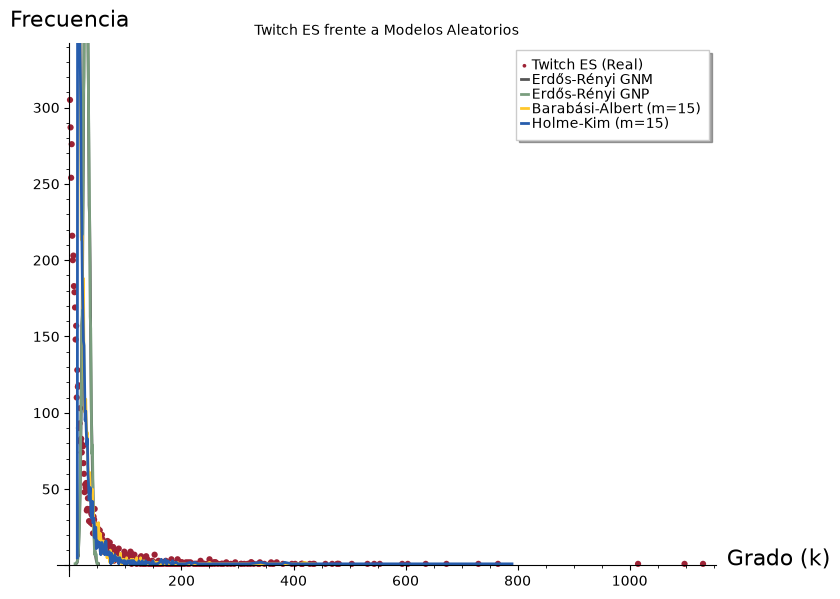
\includegraphics[width=0.60\textwidth]{datos/salidas/grafica_ES_3_modelos.png}
  \caption{Perfil de grados de Twitch en español (\texttt{ES}, 2018) frente a \texttt{GNM}, \texttt{GNP}, Barabási--Albert y Holme--Kim ($m = 15$).}
  \label{fig:modelos_es}
\end{figure}

% ==============================================================================
\section{Mundo Pequeño, Centro, las 5 Centralidades y Robustez}
% ==============================================================================

\subsection{Invariancia del Mundo Pequeño y diferencia entre Centro y Cercanía}
Comparar \texttt{PT} con \texttt{ES} verifica empíricamente el fenómeno de \textbf{Mundo Pequeño} (Watts y Strogatz, 1998)~\cite{watts1998}. Aunque la comunidad hispanohablante multiplica por $2,25$ el número de usuarios de la lusófona y reduce su densidad a menos de la mitad, la distancia media estimada mediante búsqueda en anchura (BFS desde $150$ orígenes reproducibles, preferida al algoritmo de Dijkstra~\cite{dijkstra1959} por tratarse de grafos no ponderados donde BFS opera en $O(|V|+|A|)$) apenas sube de $2,641$ a $2,872$ saltos y el diámetro pasa de $7$ a $8$. Al combinar distancias tan cortas como un grafo aleatorio (\texttt{GNP}, $2,61$) con un \textit{clustering} $22,3\times$ (\texttt{PT}) y $40,9\times$ (\texttt{ES}) superior al azar, se confirma la existencia de atajos estructurales y fuerte agrupamiento local.

En ambas componentes gigantes se cumple la desigualdad métrica $\text{rad}(G) \le \text{diam}(G) \le 2\,\text{rad}(G)$, obteniendo $4 \le 7 \le 8$ en \texttt{PT} y la igualdad extrema $4 \le 8 = 2 \cdot 4$ en \texttt{ES}. Además, el subgrafo \texttt{ES} ilustra con gran claridad la diferencia entre \textbf{Centro} y \textbf{Cercanía}. Su centro $Z(G_{\text{gig, ES}})$ se reduce a solo \textbf{$4$ vértices} (\texttt{25951}, \texttt{143506}, \texttt{49942} y \texttt{70486}), de modo que \textbf{$4$ de los $5$ usuarios con mayor Cercanía (\texttt{31958}, \texttt{151558}, \texttt{151200} y \texttt{112472}) quedan fuera del Centro} por tener excentricidad $5$. Mientras el Centro optimiza el \textit{peor caso} (basta un único vértice periférico alejado para penalizar la excentricidad), la Cercanía optimiza la distancia \textit{promedio} al resto de la red.

\subsection{Las cinco centralidades y validación con atributos reales}
El cruce de las cinco centralidades (\textbf{Grado, Cercanía, Intermediación, Autovector y Bonacich}) con los atributos reales de SNAP 2018 confirma que la topología predice el rendimiento real de los canales:
\begin{itemize}[leftmargin=*, itemsep=2pt]
  \item \textbf{Correlación de Spearman:} El grado topológico correlaciona positivamente con las visualizaciones acumuladas (\texttt{views}, $\rho = +0,5994$ en \texttt{PT} y $\rho = +0,5627$ en \texttt{ES}, $p < 10^{-200}$) y negativamente con el abandono (\texttt{dead\_account}, $\rho = -0,2061$ en \texttt{PT} y $-0,1294$ en \texttt{ES}).
  \item \textbf{Líderes frente a conectores puros en \texttt{PT}:} El nodo \texttt{122266} (grado $880$, $32,67$\,M de visitas) lidera en Grado, Cercanía ($0,5806$), Autovector ($0,1678$) y Bonacich ($0,2047$), mientras \texttt{161540} (grado $849$, $36,93$\,M de visitas) encabeza la Intermediación ($0,0889$). Sin embargo, la Intermediación rescata un \textbf{puente estructural oculto}, el usuario \texttt{102521}, que entra en el Top~10 de puentes ($0,0181$) con solo $172$ contactos y sin estatus de afiliado.
  \item \textbf{El acierto de Bonacich en \texttt{ES}:} Los dos mayores \textit{hubs} por grado e intermediación (\texttt{25951} con $1\,131$ contactos y \texttt{31958} con $1\,098$) desaparecen del Top~5 de \textbf{Autovector}, liderado por \texttt{151558} ($0,1614$). Al calcular la \textbf{centralidad de Bonacich} resolviendo $(I - \alpha A)\mathbf{c} = A\mathbf{1}$ con $\alpha = 0,5/\lambda_{\max} = 0,00436$ ($\lambda_{\max} = 114,77$), el primer puesto recae exactamente en \texttt{151558} ($0,1764$), que resulta ser el canal con mayor audiencia real del Top~5 de \texttt{ES} ($30,55$\,M de visitas frente a los $24,71$\,M de \texttt{25951} y $18,20$\,M de \texttt{31958}).
\end{itemize}

\subsection{Experimento de robustez: fallo aleatorio frente a ataque dirigido}
Para evaluar la resiliencia estructural de ambas redes, simulamos la eliminación de $20$ nodos en $G_{\text{gig}}$ bajo tres escenarios:
\begin{itemize}[leftmargin=*, itemsep=2pt]
  \item \textbf{Fallo aleatorio ($20$ nodos):} En \texttt{ES}, la red ni siquiera se desconecta (permanece en $1$ única componente de $5\,504$ nodos), y en \texttt{PT} apenas se fragmenta en $3$ componentes ($2\,420$ nodos en la gigante).
  \item \textbf{Ataque al núcleo (Top~20 Autovector):} Desconecta $27$ componentes en \texttt{ES} ($5\,478$ en la gigante) y $34$ en \texttt{PT} ($2\,387$).
  \item \textbf{Ataque a puentes (Top~20 Intermediación):} Multiplica el daño hasta \textbf{$54$ componentes en \texttt{ES}} ($5\,451$ en la gigante) y \textbf{$36$ en \texttt{PT}} ($2\,386$).
\end{itemize}
Esto confirma el comportamiento propio de las redes heterogéneas, caracterizado por una alta tolerancia a fallos aleatorios, un núcleo denso muy redundante y una vulnerabilidad concentrada en los puentes que sujetan las ramas periféricas.

% ==============================================================================
\section{Comunidades, cliques y complejidad computacional}
% ==============================================================================

La presencia de $262\,853$ triángulos ($C_3$) en \texttt{PT} y $400\,497$ en \texttt{ES} demuestra inmediatamente que ninguna de las dos redes es bipartita ($\chi(G) > 2$). Encontrar el clique máximo global es un problema \textbf{NP-Completo} (reducible en tiempo polinomial desde \texttt{3-SAT}); por ello acotamos la búsqueda exacta al núcleo de los $150$ vértices de mayor grado, hallando en ambos idiomas un subgrafo completo de tamaño \textbf{$K_{18}$}. Este hallazgo aporta dos consecuencias teóricas directas:
\begin{enumerate}[leftmargin=*, itemsep=2pt]
  \item El \textbf{número cromático} cumple la cota inferior $\chi(G) \ge \omega(G) \ge 18$.
  \item Al contener $K_5$ como subgrafo, el \textbf{Teorema de Kuratowski} garantiza que ninguno de los grafos es plano.
\end{enumerate}

Respecto a la estructura de comunidades, la maximización voraz (\textit{greedy}) de la modularidad sobre cada componente gigante particiona \texttt{PT} en \textbf{$15$ comunidades} ($Q = 0,2529$) y \texttt{ES} en \textbf{$31$ comunidades} ($Q = 0,3862$), evidenciando subculturas temáticas más diferenciadas dentro de la comunidad hispanohablante.

% ==============================================================================
\section{Preguntas de investigación: idiomas y evolución 2018--2026}
% ==============================================================================

\subsection{¿Cambia la estructura según el idioma? (Los 21 idiomas de SNAP)}
Al analizar los $6\,797\,557$ enlaces de la red global de 2018, comprobamos que exactamente el \textbf{$90,00\%$} conecta dos cuentas del mismo idioma, frente al \textbf{$73,31\%$} esperado bajo mezcla aleatoria. El coeficiente de \textbf{assortatividad de Newman}~\cite{newman2003} vale \textbf{$r = 0,6254$}, lo que confirma una fuerte homofilia lingüística: el idioma actúa como frontera comunitaria natural por encima de las fronteras geográficas (conectando España y Latinoamérica en \texttt{ES}, o Brasil y Portugal en \texttt{PT}).

La comparativa global de los $21$ idiomas ratifica además el efecto escala inverso entre tamaño y densidad: el \textbf{inglés (\texttt{EN})}, con $124\,411$ usuarios, presenta la menor densidad ($0,071\%$) pese a registrar el mayor grado medio ($88,17$), frente a comunidades medianas mucho más cohesionadas como el \textbf{chino (\texttt{ZH})}, con $2\,828$ usuarios y densidad del $1,698\%$, el \textbf{portugués (\texttt{PT})} ($2\,536$ usuarios, $1,336\%$) o el \textbf{español (\texttt{ES})} ($5\,699$ usuarios, $0,529\%$). En el extremo opuesto, la categoría residual \textbf{otros idiomas (\texttt{OTHER})} ($1\,429$ usuarios, $1\,250$ aislados y densidad del $0,020\%$) confirma que no forma una comunidad real, sino un cajón de sastre de lenguas minoritarias sin relación entre sí.

\subsection{Cambio de perspectiva en los datos y evolución temporal (2018--2026)}
Al comparar la red de 2018 con cortes posteriores resulta fundamental distinguir \textbf{dos paradigmas de construcción de grafo} y el cambio técnico que experimentó la plataforma:
\begin{itemize}[leftmargin=*, itemsep=2pt]
  \item \textbf{Grafo de seguimiento mutuo (SNAP 2018):} dos usuarios se enlazan si se siguen recíprocamente en sus perfiles.
  \item \textbf{Proyección bipartita de audiencia en directo (Kaggle 2019, GitHub Overlap 2021--2022 y captura propia de 2026):} se parte de un grafo bipartito $G_{\text{bip}} = (U \cup S, E)$ entre espectadores ($U$) y \textit{streamers} ($S$) que interactúan en vivo, y se proyecta sobre $S$ uniendo dos canales cuando comparten audiencia activa. En los estudios de \textbf{Kaggle 2019} (\texttt{full\_a.csv}, Rappaz et al., 2021~\cite{rappaz2021}) y \textbf{GitHub Overlap (diciembre 2021 y enero 2022)}, sus autores eligieron ya este modelo porque refleja mejor qué comunidades comparten público real en directo que las listas estáticas de seguidores. Posteriormente, en \textbf{mayo de 2022} Twitch eliminó su función social de «Amigos» (\textit{Friends}) y en \textbf{agosto de 2023} restringió el \textit{endpoint} público de seguidores de su API oficial (\textit{Helix}), haciendo imposible reconstruir desde fuera un grafo como el de 2018. Por ello, nuestra captura propia de \textbf{noviembre de 2026} (obtenida combinando la API \textit{Helix} y lectura de chats IRC para canales en \texttt{ES} y \texttt{PT}) sigue exactamente el mismo paradigma de proyección bipartita que los grafos de 2019 y 2021--2022.
\end{itemize}

Cabe preguntarse si tiene sentido comparar redes construidas de forma tan distinta. Precisamente ese contraste permite separar qué diferencias provienen de \textbf{cómo se modelan las aristas} (que explica el salto inmediato del agrupamiento local entre 2018 y 2019) y cuáles reflejan la \textbf{evolución temporal real} de la plataforma al comparar cortes del mismo paradigma entre sí (2019 frente a 2021--2022 y 2026). Al mismo tiempo, permite identificar qué invariantes estructurales (mundo pequeño, concentración en \textit{hubs} y Paradoja de la Amistad) se mantienen estables en ambos enfoques.

\begin{table}[H]
\centering
\caption{Comparativa estructural entre seguimiento mutuo (2018) y proyecciones de audiencia en directo (2019--2026).}
\label{tab:evolucion}
\setlength{\tabcolsep}{4pt}
\resizebox{\textwidth}{!}{%
\begin{tabular}{@{}lrrrrrrrrrrr@{}}
\toprule
\textbf{Corte temporal / Red} & \textbf{Nodos} & \textbf{Aristas} & \textbf{Dens.\%} & \textbf{G.\,Med} & $\mathbf{CV}$ & \textbf{Clust.} & \textbf{Dist.} & \textbf{Diam.} & \textbf{Par.\%} & \textbf{Com.} & \textbf{Cliq.} \\
\midrule
2018 SNAP (\texttt{PT}) & $2\,536$ & $42\,952$ & $1,34$ & $33,9$ & $1,84$ & $0,3031$ & $2,64$ & $7$ & $93,9$ & $15$ & $K_{18}$ \\
2018 SNAP (\texttt{ES}) & $5\,699$ & $85\,893$ & $0,53$ & $30,1$ & $1,93$ & $0,2247$ & $2,87$ & $8$ & $95,0$ & $31$ & $K_{18}$ \\
2019 Kaggle (Bruto $\ge 5$) & $1\,000$ & $65\,799$ & $13,17$ & $131,6$ & $0,84$ & $0,7278$ & $1,90$ & $3$ & $89,3$ & $4$ & $K_{75}$ \\
2019 Kaggle (Top-15) & $1\,000$ & $12\,077$ & $2,42$ & $24,2$ & $1,12$ & $0,7318$ & $2,92$ & $6$ & $87,9$ & $11$ & $K_{15}$ \\
Dic.\ 2021 Overlap (Top-15) & $1\,150$ & $7\,052$ & $1,07$ & $12,3$ & $1,26$ & $0,7291$ & $4,25$ & $10$ & $88,9$ & $17$ & $K_{13}$ \\
Ene.\ 2022 Overlap (Top-15) & $1\,682$ & $10\,950$ & $0,77$ & $13,0$ & $1,28$ & $0,6988$ & $4,50$ & $10$ & $87,4$ & $21$ & $K_{13}$ \\
Nov.\ 2026 Propia (\texttt{ES}+\texttt{PT}) & $163$ & $1\,015$ & $7,69$ & $12,5$ & $0,85$ & $0,4651$ & $2,79$ & $9$ & $79,6$ & $7$ & $K_{11}$ \\
\bottomrule
\end{tabular}%
}
\end{table}

La Tabla~\ref{tab:evolucion} permite extraer tres conclusiones estructurales de los conjuntos históricos:
\begin{enumerate}[leftmargin=*, itemsep=2pt]
  \item \textbf{Salto constructivo en Clustering por proyección bipartita ($0,22\text{--}0,30 \to 0,70\text{--}0,73$):} Que el grafo de \textbf{2019}, separado por solo un año del de 2018, alcance ya un \textit{clustering} de $0,7318$ demuestra que este salto no se debe a un cambio repentino de los usuarios, sino a la geometría de la proyección. Cada grupo de espectadores que participa en $k$ canales induce automáticamente un clique $K_k$ con $\binom{k}{2}$ aristas lleno de triángulos.
  \item \textbf{Efecto de la saturación y necesidad de poda:} En Kaggle 2019 sin límite de enlaces por nodo ($\ge 5$ espectadores comunes), la red se satura ($13,17\%$ de densidad, $4$ comunidades y un clique gigante $K_{75}$). Aplicar la poda \texttt{Top-15} (conservando las $15$ conexiones de mayor peso por canal, igual que en 2021--2022 y 2026) recupera una red dispersa comparable ($11$ comunidades, diámetro $6$) preservando intacto el \textit{clustering} ($0,7318$).
  \item \textbf{Evolución temporal entre 2019 y 2022:} Mientras en 2019 la red de audiencia estaba dominada por grandes creadores anglosajones de \textit{Fortnite} y \textit{shooters} (\texttt{shroud}, \texttt{ninja}, \texttt{tfue}), en enero de 2022 se produce un contraste muy ilustrativo entre centralidades. El canadiense \texttt{xqcow} lidera globalmente en Grado ($246$) e Intermediación ($0,3645$), acompañado como puentes internacionales por canales de \textit{esports} (\texttt{s1mple}, \texttt{lec} y \texttt{lck\_korea}), pero \textbf{el Top~5 mundial de Autovector pasa a ser íntegramente hispanohablante}, encabezado por \texttt{ibai} ($0,2721$), \texttt{elxokas} ($0,2663$), \texttt{thegrefg} ($0,2641$), \texttt{rubius} ($0,2468$) y \texttt{auronplay} ($0,2432$), con picos de $739\,781$ espectadores compartidos entre \texttt{ibai} y \texttt{thegrefg}. Aunque \texttt{xqcow} enlaza con más canales dispersos, la cohesión interna del bloque hispanohablante concentra el autovector dominante de la plataforma.
\end{enumerate}

\subsection{Validación experimental propia en tiempo real (noviembre de 2026)}
Para comprobar si los patrones estructurales identificados en los conjuntos históricos siguen vigentes ocho años después de SNAP 2018, diseñamos e implementamos una captura propia en tiempo real durante tres noches consecutivas de noviembre de 2026 (viernes, sábado y domingo en franja de máxima audiencia, dos horas por sesión). Mediante la API oficial \textit{Helix} de Twitch identificamos cada noche los $50$ directos con mayor audiencia en \texttt{ES} y los $50$ mayores en \texttt{PT}, y nos conectamos de forma simultánea a sus chats mediante el protocolo IRC (gestionando el límite de ritmo de \texttt{JOIN} por tandas sin bloquear la lectura ni perder mensajes).

A partir de los usuarios únicos registrados en cada chat construimos la proyección bipartita exigiendo al menos $2$ espectadores compartidos por enlace para filtrar coincidencias puntuales (obteniendo $1\,055$ aristas brutas) y aplicamos la misma poda \texttt{Top-15} utilizada en 2021 y 2022. El grafo resultante cuenta con \textbf{$163$ canales y $1\,015$ aristas}, sin nodos aislados y con una componente conexa gigante de $157$ vértices ($96,3\%$).

\begin{table}[H]
\centering
\caption{Top~5 de canales según Grado, Intermediación y Autovector en nuestra captura propia (noviembre de 2026).}
\label{tab:top_2026}
\small
\begin{tabular}{@{}clrlrlr@{}}
\toprule
\textbf{Pos.} & \textbf{Grado} & \textbf{Valor} & \textbf{Intermediación} & \textbf{Valor} & \textbf{Autovector} & \textbf{Valor} \\
\midrule
1 & \texttt{peereira7} & $55$ & \texttt{werlyb} & $0,1156$ & \texttt{peereira7} & $0,2640$ \\
2 & \texttt{rubius} & $52$ & \texttt{kennzy} & $0,0954$ & \texttt{rubius} & $0,2512$ \\
3 & \texttt{djmariio} & $49$ & \texttt{peereira7} & $0,0903$ & \texttt{djmariio} & $0,2350$ \\
4 & \texttt{thegrefg} & $45$ & \texttt{djmariio} & $0,0820$ & \texttt{thegrefg} & $0,2223$ \\
5 & \texttt{illojuan} & $42$ & \texttt{podrecdd} & $0,0754$ & \texttt{auronplay} & $0,2181$ \\
\bottomrule
\end{tabular}
\end{table}

Los resultados de esta muestra propia confirman tres hipótesis clave del trabajo:
\begin{itemize}[leftmargin=*, itemsep=2pt]
  \item \textbf{Persistencia de la frontera lingüística:} De los $1\,055$ enlaces capturados entre los canales de \texttt{ES} y \texttt{PT}, exactamente $937$ unen canales del mismo idioma (\textbf{$88,82\%$}). Esta cifra replica casi con exactitud el $90,00\%$ observado en SNAP 2018, demostrando que la segregación lingüística se mantiene estable pese al paso de ocho años y al cambio en la definición de arista (Figura~\ref{fig:red_2026}).
  \item \textbf{Coherencia topológica a escala de ventana corta:} La red mantiene un comportamiento de mundo pequeño ($2,79$ saltos de distancia media y diámetro $9$), un núcleo denso de tamaño $K_{11}$, $7$ comunidades diferenciadas y un $79,6\%$ de afectación por la Paradoja de la Amistad. Su \textit{clustering} ($0,4651$) supera claramente al de las redes de seguimiento de 2018 ($0,22\text{--}0,30$), confirmando el efecto de la proyección bipartita, aunque se sitúa por debajo de los cortes mensuales de 2019--2022 ($0,70\text{--}0,73$) porque una ventana de tres noches registra menos saltos simultáneos de un mismo espectador entre muchos canales.
  \item \textbf{Separación real de roles en las centralidades (Tabla~\ref{tab:top_2026}):} Mientras el Grado y el Autovector quedan en manos del gran bloque de entretenimiento hispanohablante (\texttt{peereira7}, \texttt{rubius}, \texttt{djmariio}, \texttt{thegrefg}, \texttt{illojuan} y \texttt{auronplay}), la \textbf{Intermediación} da un giro completo y coloca en cabeza a \texttt{werlyb} ($0,1156$, creador de \textit{League of Legends} en \texttt{ES}), \texttt{kennzy} ($0,0954$, comunidad competitiva en \texttt{PT}) y \texttt{podrecdd} ($0,0754$, comunidad en \texttt{PT}). Esto demuestra sobre datos en directo que los videojuegos competitivos internacionales actúan como los puentes efectivos entre comunidades lingüísticas distintas.
\end{itemize}

\begin{figure}[H]
  \centering
  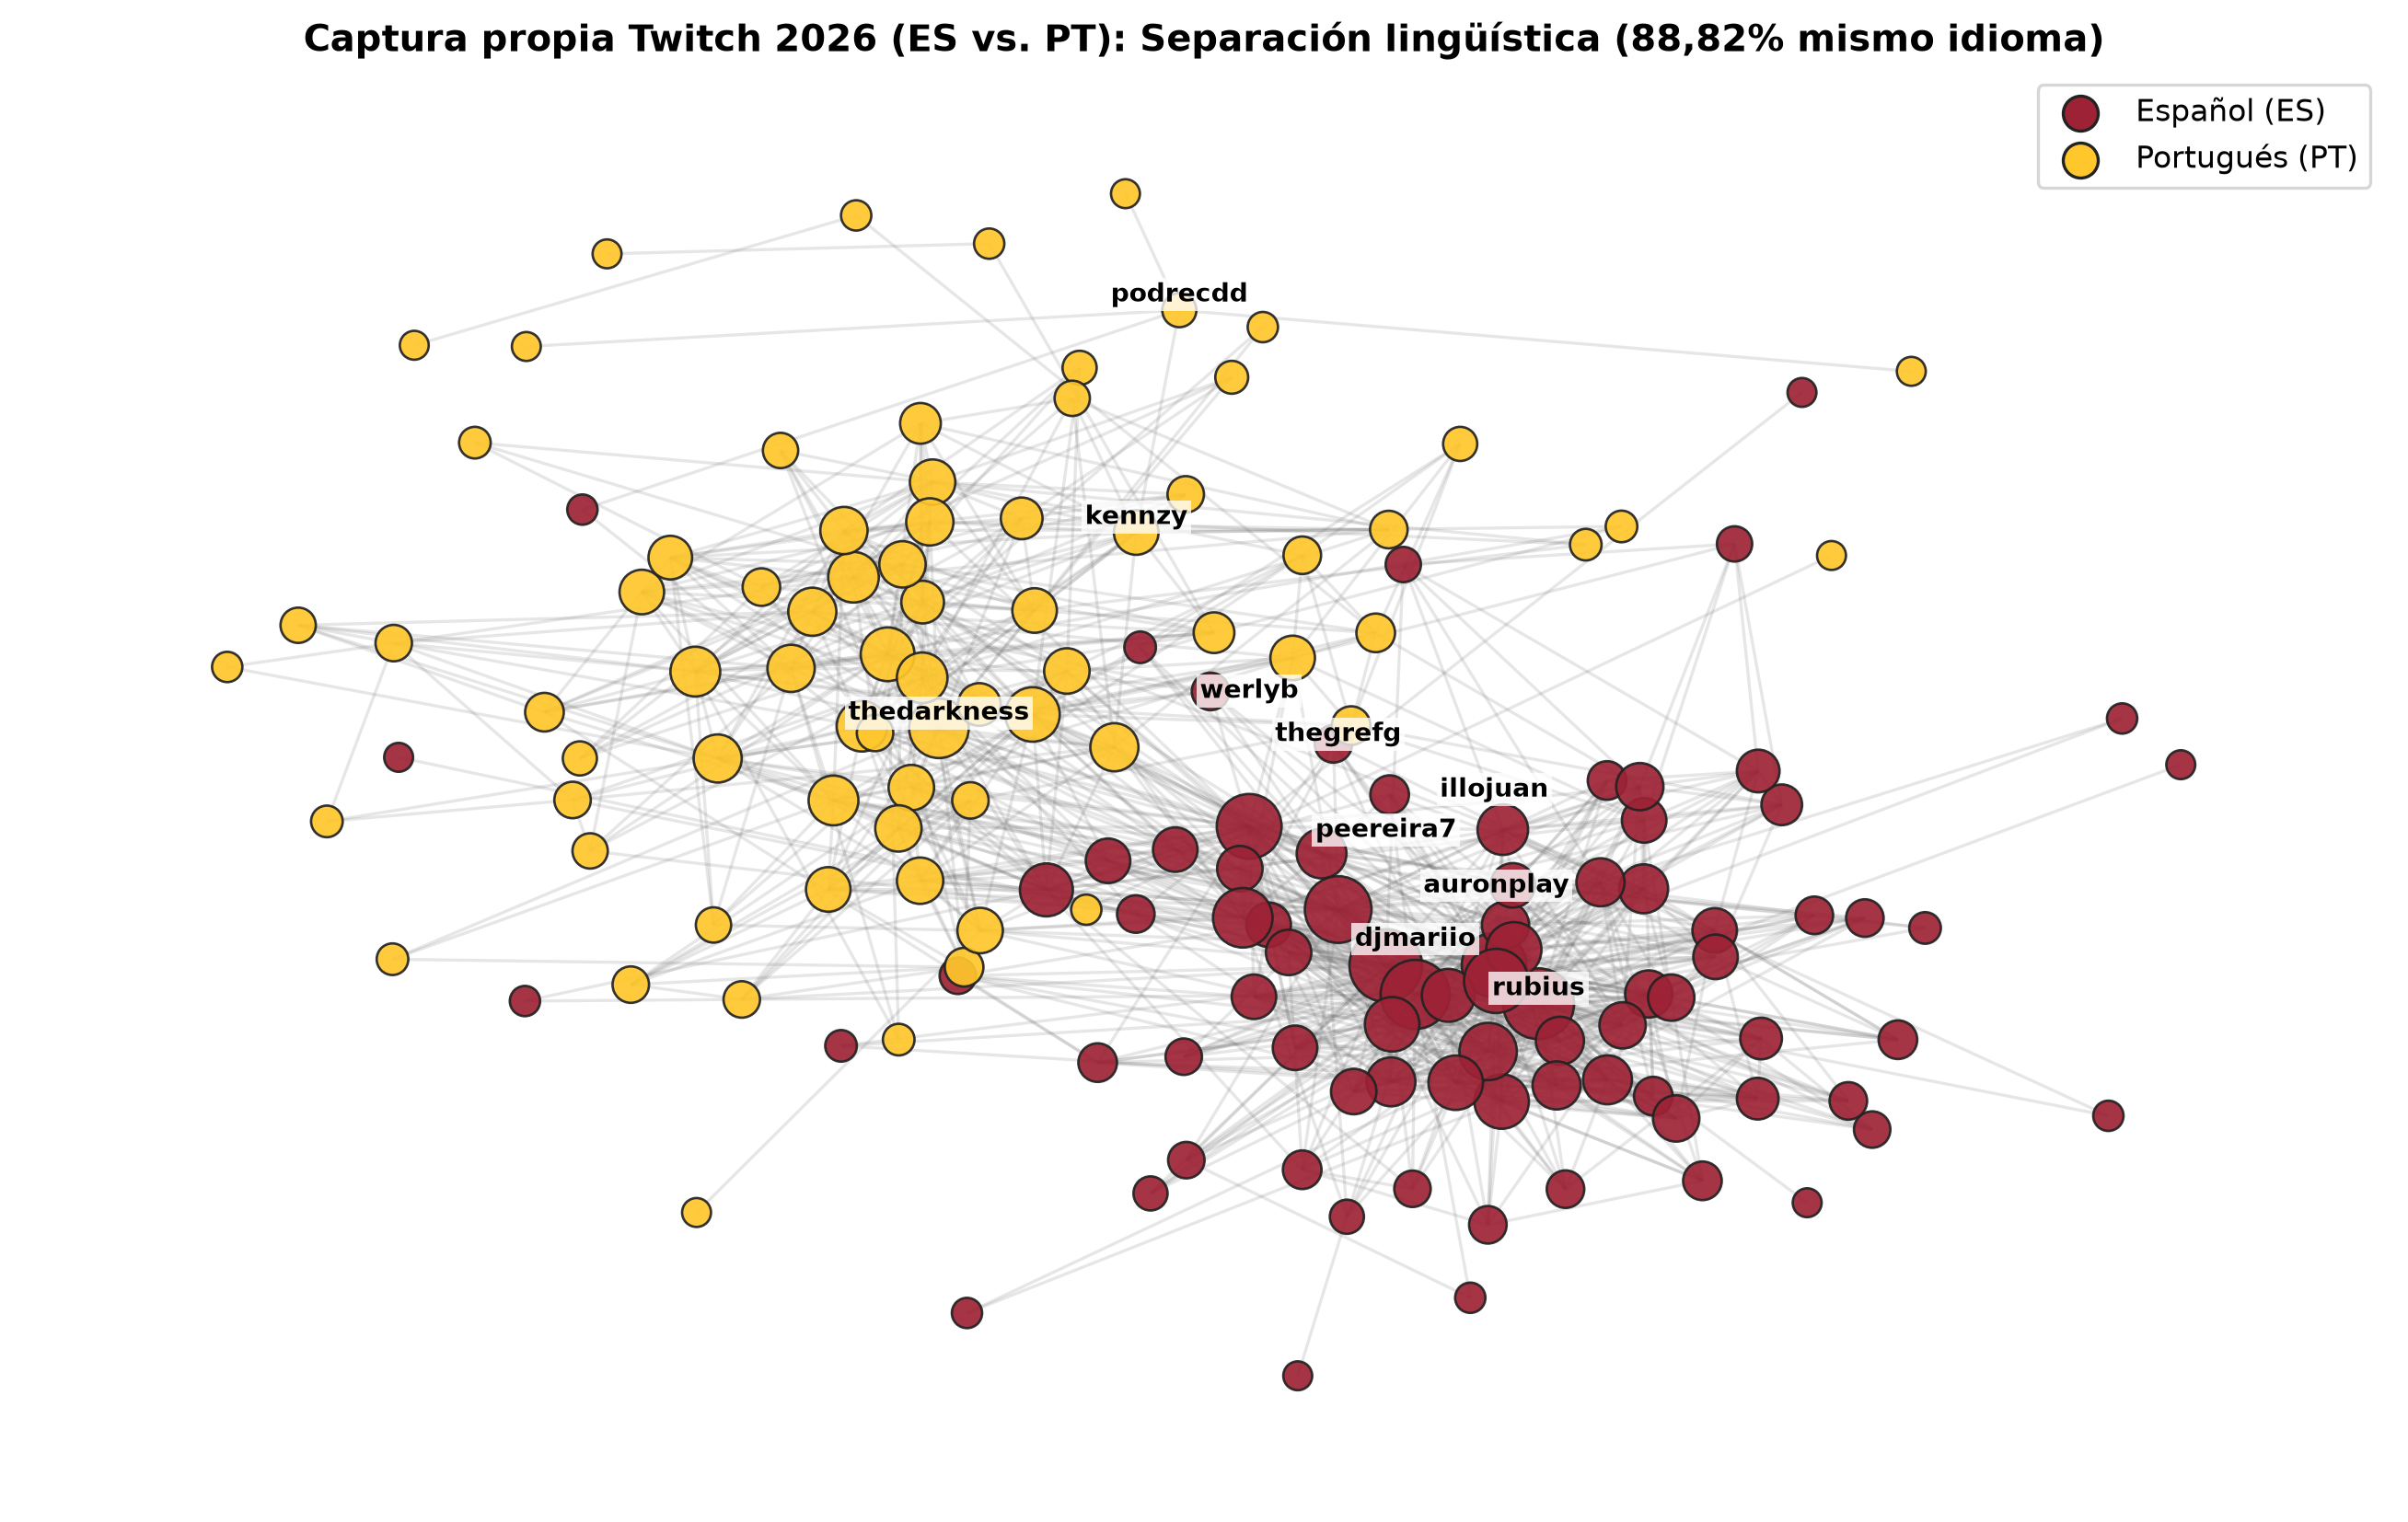
\includegraphics[width=0.66\textwidth]{datos/salidas/grafica_red_2026.png}
  \caption{Red capturada en directo en noviembre de 2026 (\texttt{ES} en burdeos y \texttt{PT} en albero), donde se aprecia la segregación lingüística ($88,82\%$ de aristas internas) y los puentes competitivos entre bloques.}
  \label{fig:red_2026}
\end{figure}

% ==============================================================================
\section{Demostraciones constructivas y aplicación divulgativa}
% ==============================================================================

Para ilustrar de forma verificable los fundamentos algorítmicos del trabajo, realizamos dos comprobaciones constructivas paso a paso:
\begin{itemize}[leftmargin=*, itemsep=2pt]
  \item \textbf{Reducción de Havel--Hakimi sobre la cúpula de \texttt{ES} 2018~\cite{hakimi1962}:} Extraemos el subgrafo inducido por los $6$ mayores \textit{hubs} (\texttt{25951}, \texttt{31958}, \texttt{151558}, \texttt{8555}, \texttt{151200} y \texttt{49235}), verificamos que su matriz de adyacencia es cuadrada, simétrica y de diagonal nula, y reducimos constructivamente su secuencia de grados:
  \[
    [5,5,3,3,2,2] \longrightarrow [4,2,2,1,1] \longrightarrow [1,1,0,0] \longrightarrow [0,0,0].
  \]
  Esto confirma que la secuencia es gráfica y revela que los dos líderes de grado $5$ están conectados entre sí y con todos los demás miembros de la cúpula. De igual modo, en los $6$ mayores \textit{hubs} de \texttt{PT} la secuencia $[4,4,4,4,4,2]$ se reduce en cuatro pasos a $[0,0]$.
  \item \textbf{Partición constructiva de Girvan--Newman:} Sobre un grafo didáctico de $8$ vértices compuesto por dos bloques densos unidos por una única arista puente $(3,4)$, el cálculo exacto de intermediación de aristas asigna $4 \times 4 = 16,0$ caminos mínimos a $(3,4)$ (frente a un máximo de $7,5$ en las demás). Su eliminación divide inmediatamente el grafo en dos comunidades de tamaño $4$ (Figura~\ref{fig:girvan}).
\end{itemize}

\begin{figure}[H]
  \centering
  \begin{subfigure}[b]{0.40\textwidth}
    \centering
    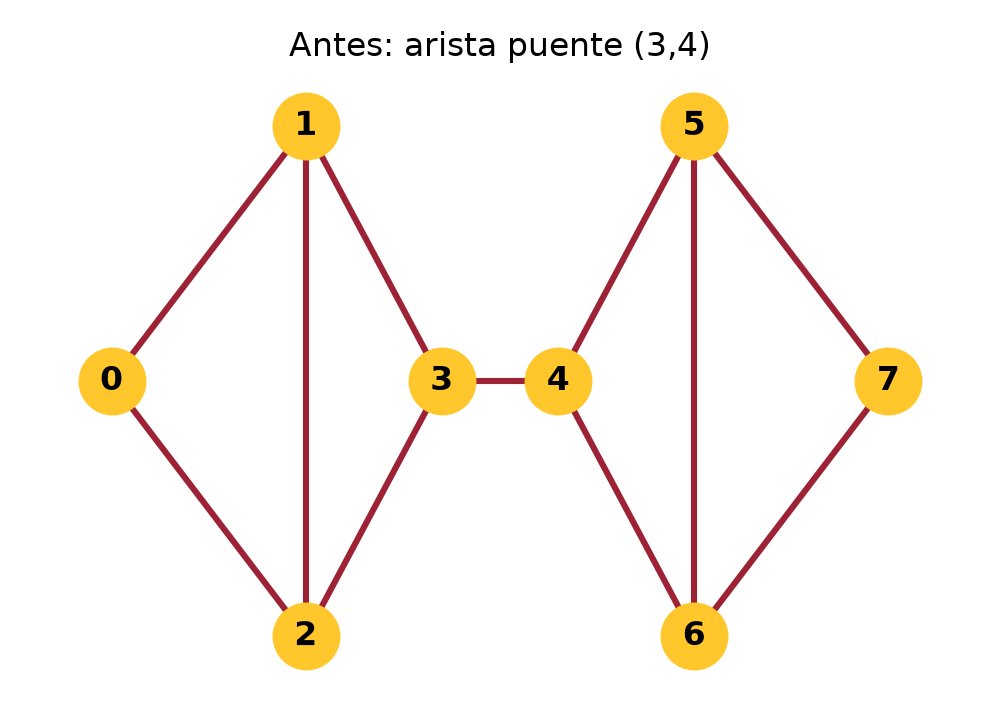
\includegraphics[width=\textwidth]{datos/salidas/grafica_4a_girvan_antes.png}
    \caption{Grafo inicial con arista puente $(3,4)$.}
  \end{subfigure}
  \hfill
  \begin{subfigure}[b]{0.40\textwidth}
    \centering
    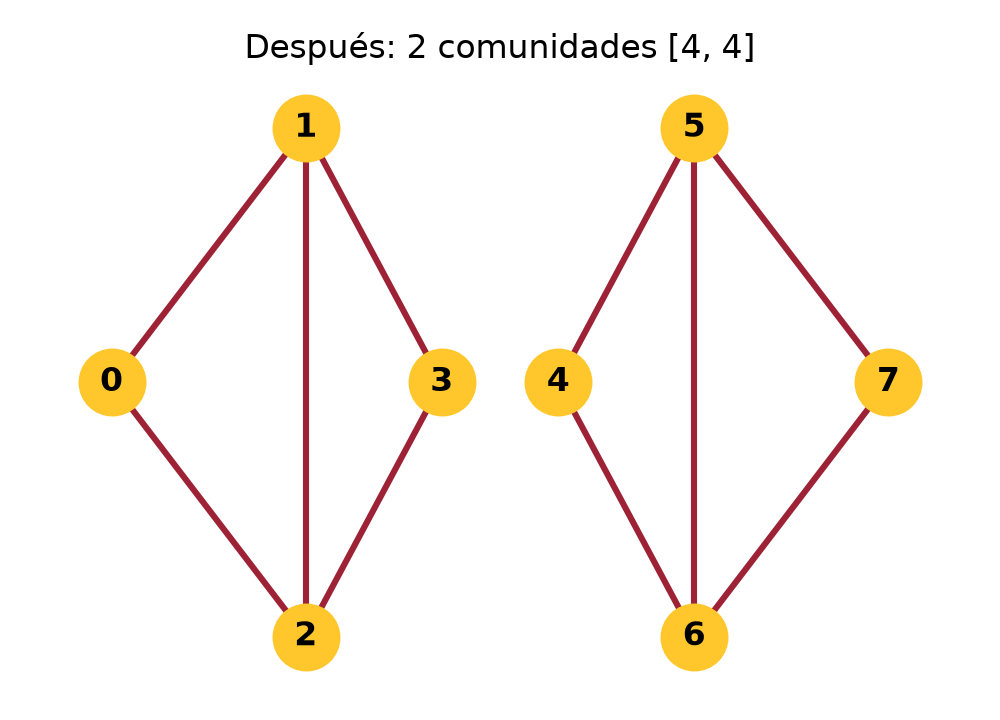
\includegraphics[width=\textwidth]{datos/salidas/grafica_4b_girvan_despues.png}
    \caption{Partición en dos comunidades $[4,4]$.}
  \end{subfigure}
  \caption{Demostración constructiva de una iteración del algoritmo de Girvan--Newman.}
  \label{fig:girvan}
\end{figure}

Como complemento divulgativo, hemos desarrollado la aplicación web interactiva \texttt{app\_twitch.py} en \textit{Streamlit}. La herramienta permite alternar en tiempo real entre los datasets (2018--2026), explorar visualmente las comunidades y rankings de cada medida de centralidad, simular fallos aleatorios o ataques dirigidos sobre \textit{hubs} y puentes, y ejecutar en vivo las demostraciones constructivas de Girvan--Newman, proyección bipartita y Havel--Hakimi.

% ==============================================================================
\section{Trazabilidad y verificación crítica del uso de la IA}
% ==============================================================================

Siguiendo el protocolo de transparencia de la asignatura, el grupo ha empleado herramientas de inteligencia artificial como asistente técnico de programación y apoyo metodológico, manteniendo en todo momento el diseño del estudio, la comprobación de hipótesis y la validación crítica de los resultados:
\begin{enumerate}[leftmargin=*, itemsep=2pt]
  \item \textbf{Planteamiento y base propia:} El diseño del proyecto, la formulación de las preguntas de investigación y el análisis base se construyeron a partir de los conceptos y funciones trabajados en las prácticas de MATI~\cite{reyes2026} (\texttt{degree\_\allowbreak sequence}, \texttt{find\_\allowbreak fit}, modelos \texttt{GNM}/\texttt{GNP}/\texttt{BA}/\texttt{HK}, \texttt{centrality\_\allowbreak betweenness} y \texttt{centrality\_\allowbreak closeness}). Sobre esa base definimos qué invariantes calcular, qué comprobaciones previas exigir (conexidad, Lema del apretón de manos, Teorema de Whitney) y cómo contrastar las redes de 2018 con cortes más recientes.
  \item \textbf{Uso dirigido de la IA:} Recurrimos a IA generativa (Gemini) mediante consultas técnicas concretas (por ejemplo, solicitando cómo resolver el sistema lineal de Bonacich en formato disperso sin desbordar la memoria o cómo gestionar las restricciones de la API \textit{Helix} y los límites de conexión de IRC) para agilizar el procesamiento de los $6,79$\,M de aristas, las proyecciones bipartitas (2019--2026) y la interfaz en \textit{Streamlit} de \texttt{app\_twitch.py}.
  \item \textbf{Verificación crítica y correcciones realizadas por el equipo:} Todo código y resultado generado se revisó matemáticamente y se contrastó con ejecuciones reales, detectando y corrigiendo cinco incidencias relevantes:
  \begin{itemize}[leftmargin=*, itemsep=1pt]
    \item \textit{Centralidad de autovector y orden de vértices en Bonacich:} Un primer fragmento invocaba \texttt{eigenvector\_\allowbreak centrality()} directamente sobre un objeto \texttt{Graph} de \textit{SageMath}, provocando \texttt{AttributeError}. Lo corregimos convirtiendo a \textit{NetworkX} y, al implementar Bonacich, forzamos explícitamente \texttt{sorted()} sobre la lista de vértices para asegurar que cada fila de la matriz de adyacencia correspondiera al usuario correcto.
    \item \textit{Truncamiento artificial en modelos aleatorios:} Detectamos que un tope preliminar $m_{\text{modelo}} = \min(10, \text{round}(m/n))$ generaba grafos \texttt{BA} y \texttt{HK} con $25\,260$ aristas frente a las $42\,952$ reales de \texttt{PT}, falseando la comparación. Al eliminarlo ($m = 17$ en \texttt{PT} y $m = 15$ en \texttt{ES}) se igualó exactamente el grado medio real.
    \item \textit{Conflictos con el preprocesador de SageMath:} Corregimos el uso de la variable \texttt{D} (reservada al operador derivada \texttt{DerivativeOperator}), la conversión explícita con \texttt{float()} e \texttt{int()} para evitar fallos con tipos \texttt{Rational} y \texttt{RealLiteral}, y la protección de dominio en \texttt{find\_fit} mediante \texttt{abs(x - c)\textasciicircum b}.
    \item \textit{Datación real y saturación del dataset de Kaggle:} Al inspeccionar los \textit{hubs} de \texttt{full\_a.csv} (\texttt{ninja}, \texttt{shroud}, \texttt{tfue}), advertimos que aunque el archivo se alojó en Kaggle en 2023, correspondía realmente a interacciones de 2019, y comprobamos que sin aplicar la poda \texttt{Top-15} la proyección bipartita satura la red ($13,17\%$, $K_{75}$).
    \item \textit{Saturación del búfer IRC en la captura de 2026:} La primera versión enviaba pausas bloqueantes entre comandos \texttt{JOIN} sin leer mensajes entrantes, provocando cortes del servidor (\texttt{ConnectionResetError}). Lo resolvimos implementando unión por tandas no bloqueante (respetando el límite de Twitch), autoguardado periódico y reconexión automática.
  \end{itemize}
  \item \textbf{Ampliación del alcance:} Más allá del artículo original, ampliamos el análisis con el contraste completo entre \texttt{PT} y \texttt{ES} en 2018, el estudio de assortatividad sobre los $21$ idiomas, la evolución temporal 2018--2026 con datos propios capturados en directo, las simulaciones de ataque dirigido y la aplicación divulgativa interactiva.
\end{enumerate}
\newpage
% ==============================================================================
\section{Conclusiones}
% ==============================================================================

El estudio confirma que las redes de Twitch exhiben una topología de \textbf{mundo pequeño invariante de escala} (diámetro entre $7$ y $8$ saltos al duplicar la población, con un agrupamiento de $22\times$ a $41\times$ superior al azar), una desigualdad extrema que dispara la \textbf{Paradoja de la Amistad} hasta el $94\text{--}95\%$ en 2018 y una marcada \textbf{segregación lingüística} que permanece estable durante ocho años ($90,00\%$ de aristas intralingüísticas y $r = 0,6254$ en SNAP 2018, y $88,82\%$ en nuestra captura propia de 2026).

Asimismo, hemos comprobado que las distintas medidas de centralidad identifican roles reales diferentes, desde la validación de \texttt{views} mediante Bonacich en \texttt{ES} 2018 hasta los puentes competitivos \texttt{werlyb} y \texttt{kennzy} entre comunidades en 2026. Por último, separar el impacto del cambio de definición de arista (seguimiento mutuo frente a proyecciones bipartitas, que dispara el \textit{clustering} por inducción de cliques) de la evolución temporal dentro de un mismo paradigma permite explicar con rigor fenómenos reales como el auge del bloque hispanohablante en enero de 2022.

% ==============================================================================
\begin{thebibliography}{99}
\small
\setlength{\itemsep}{2pt}
\setlength{\parskip}{0pt}
% ==============================================================================

\bibitem{barabasi1999}
Barabási, A.-L., \& Albert, R. (1999). Emergence of scaling in random networks. \textit{Science}, 286(5439), 509--512.

\bibitem{clauset2009}
Clauset, A., Shalizi, C.~R., \& Newman, M.~E.~J. (2009). Power-Law Distributions in Empirical Data. \textit{SIAM Review}, 51(4), 661--703.

\bibitem{dijkstra1959}
Dijkstra, E.~W. (1959). A note on two problems in connexion with graphs. \textit{Numerische Mathematik}, 1(1), 269--271.

\bibitem{hakimi1962}
Hakimi, S.~L. (1962). On realizability of a set of integers as degree sequences of the vertices of a graph. \textit{J.\ SIAM}, 10(3), 496--506.

\bibitem{holme2002}
Holme, P., \& Kim, B.~J. (2002). Growing scale-free networks with tunable clustering. \textit{Physical Review E}, 65(2), 026107.

\bibitem{newman2003}
Newman, M.~E.~J. (2003). Mixing patterns in networks. \textit{Physical Review E}, 67(2), 026126.

\bibitem{rappaz2021}
Rappaz, J., McAuley, J., \& Aberer, K. (2021). Recommendation on Live-Streaming Platforms: Dynamic Availability and Repeat Consumption. \textit{Proc.\ 15th ACM Conference on Recommender Systems (RecSys '21)}, 390--399.

\bibitem{reyes2026}
Reyes, P., \& Garijo, D. (2026). \textit{Repaso de Matemática Discreta y Teoría de Grafos (MATI)}. Dpto.\ de Matemática Aplicada I, Universidad de Sevilla.

\bibitem{rozemberczki2021}
Rozemberczki, B., \& Sarkar, R. (2021). Twitch Gamers: a Dataset for Evaluating Proximity Preserving and Structural Role-based Node Embeddings. \textit{arXiv:2101.03091} (SNAP, Stanford University).

\bibitem{watts1998}
Watts, D.~J., \& Strogatz, S.~H. (1998). Collective dynamics of `small-world' networks. \textit{Nature}, 393(6684), 440--442.

\end{thebibliography}

\end{document}